\documentclass[14pt,xcolor=dvipsnames]{beamer}
\setbeamercolor{structure}{fg=Orange!95!black}
\usetheme{Madrid}

\usepackage{graphicx}
\graphicspath{ {images/} }

% Hide navigation symbols
\setbeamertemplate{navigation symbols}{}

\title[Stroke width on image segmentation]{Effects of stroke width on semi-automatic image segmentation}
\author[Katrina Hoffert, Mark Eramian]{Katrina Hoffert \\ Under the supervision of Dr Mark Eramian}
\date{2016-2017}

\begin{document}

\begin{frame}[plain]
	\titlepage
\end{frame}
\addtocounter{framenumber}{-1}

\begin{frame}[fragile,t]{Semi-automatic image segmentation}
	\begin{itemize}
		\item The goal of image segmentation is to portion an image into distinct segments.
		\item Semi-automatic image segmentation uses some degree of user interaction to assist in this segmentation.
		\item The method of user interaction used in our study is users annotating what is foreground and what is background.
	\end{itemize}
\end{frame}

\begin{frame}[fragile,t]{Segmentation example}
	\begin{center}
		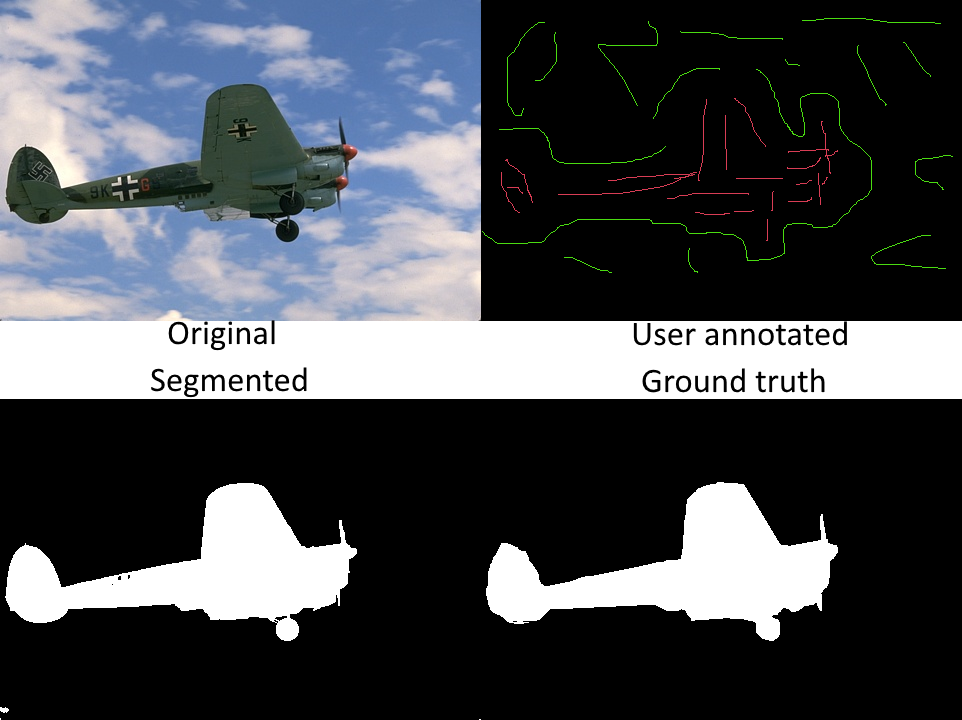
\includegraphics[width=\paperheight]{example_combined}
	\end{center}
\end{frame}

\begin{frame}[fragile,t]{Data sources}
	\begin{itemize}
		\item Images used and their ground truths all come from the Berkeley Segmentation Data Set and Benchmarks 500 (BSDS500).
	\end{itemize}
	\begin{center}
		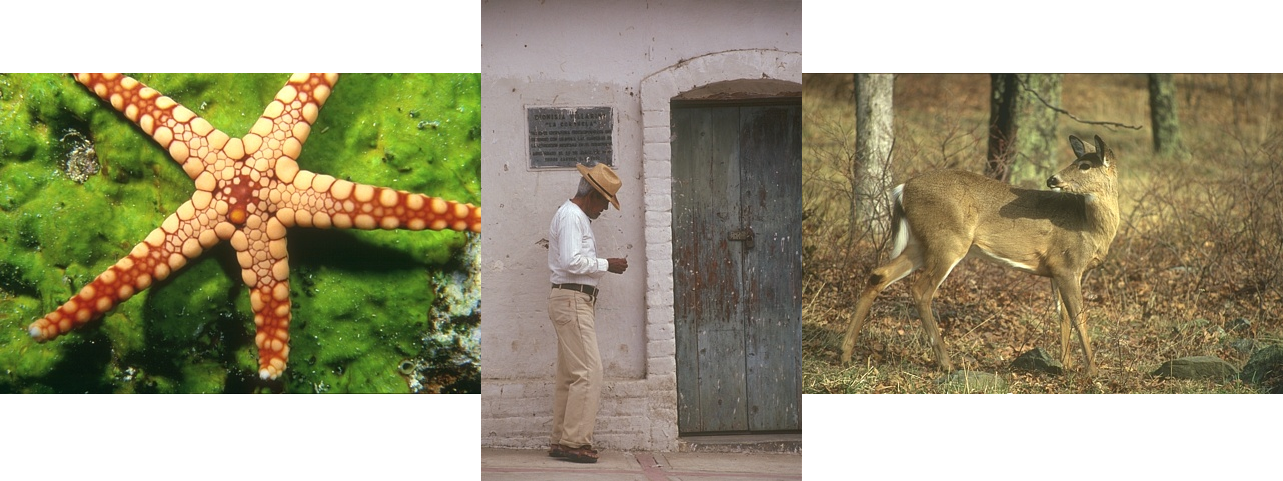
\includegraphics[width=\paperheight]{bsds500_samples}
	\end{center}
\end{frame}

\begin{frame}[fragile,t]{Data sources}
	\begin{itemize}
		\item All data used in this study came from two prior studies:
		\begin{itemize}
			\item Steven Rau: Contrasted effectiveness of user annotations in points vs strokes.
			\item Yuanxia Li: Contrasted effect of time limits on user (used only points)
		\end{itemize}
	\end{itemize}
	\begin{center}
		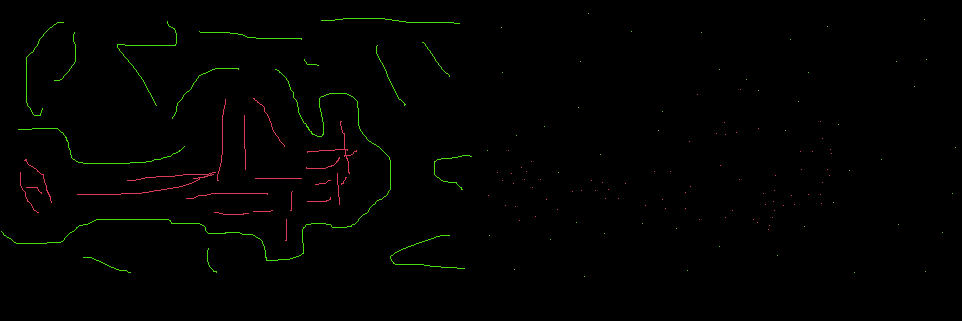
\includegraphics[width=\paperheight]{strokes_vs_points}
	\end{center}
\end{frame}

\begin{frame}[fragile,t]{Problem}
	\begin{itemize}
		\item All the data in these studies used strokes and points one pixel wide.
		\item \textbf{Question: does the width of these annotations significantly impact results?}
		\item Or in other words, can we get better results if we dilate all the annotations so that they're thicker?
		\item Supplies more data to the segmentation algorithm. But how valuable is that data? Can it introduce errors?
	\end{itemize}
\end{frame}

\begin{frame}[fragile,t]{The experiment}
	\begin{itemize}
		\item There was the worry of introducing errors that users wouldn't have made unless they were aware of the thicker stroke radius, so our dilation method only dilated if it wouldn't introduce \textit{new} errors in doing so.
		\item If an area is background (which we know because we have the ground truth), then a foreground pixel that was in the foreground wouldn't be dilated into the background.
		\item But if a foreground pixel was in the background, it would be dilated as normal.
	\end{itemize}
\end{frame}

\begin{frame}[fragile,t]{The experiment}
	\begin{center}
		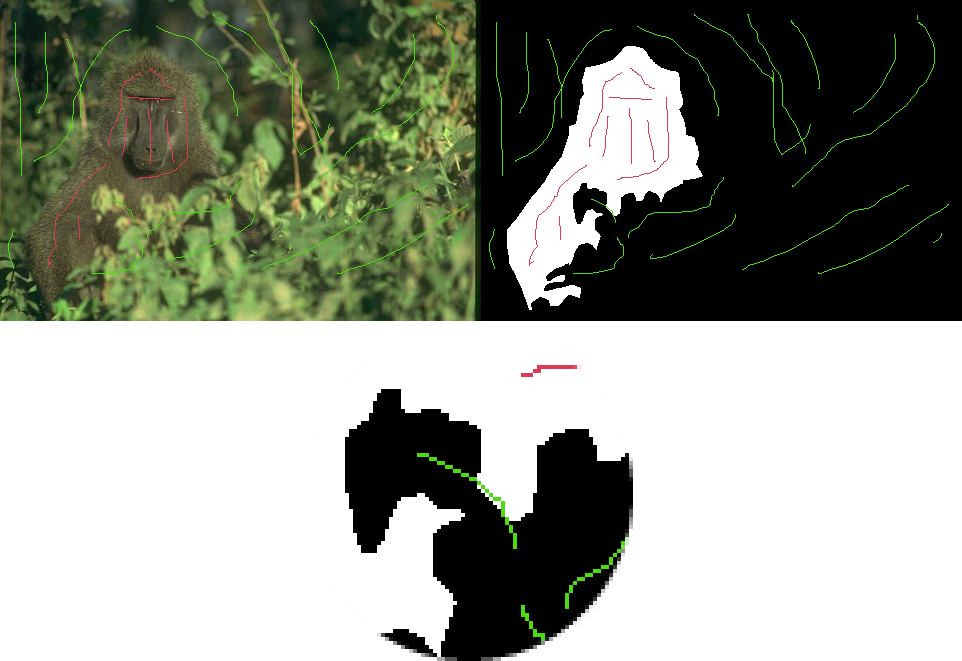
\includegraphics[width=\paperheight]{dilation_error_example}
	\end{center}
\end{frame}

\begin{frame}[fragile,t]{The experiment}
	\begin{center}
		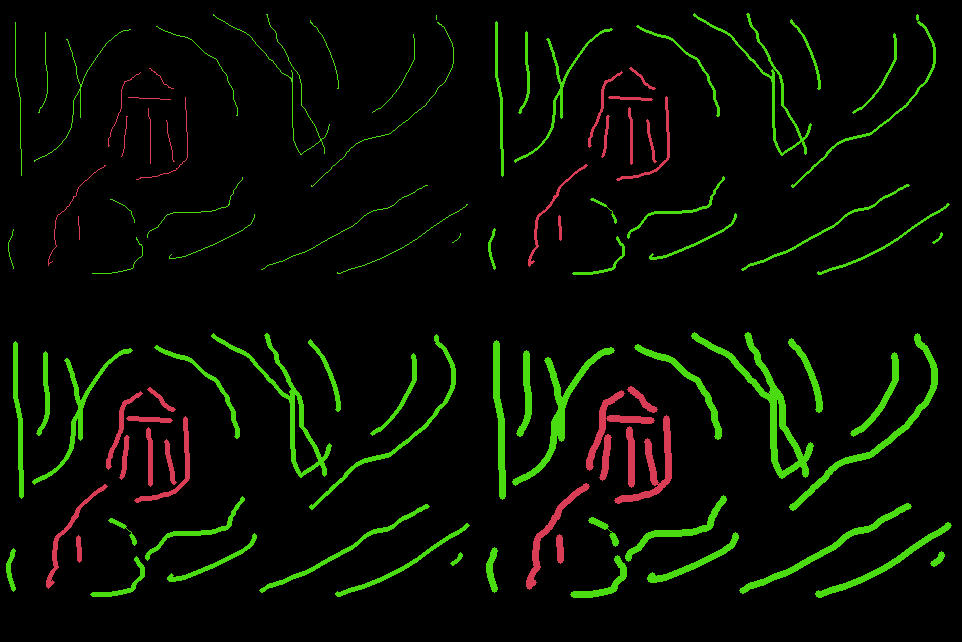
\includegraphics[width=\paperheight]{dilate_example_all}
	\end{center}
\end{frame}

\begin{frame}[fragile,t]{The experiment}
	\begin{itemize}
		\item The idea is that the strokes/points represent the center of where the user actually intended the stroke/point to be.
		\item Ultimately doesn't seem to make a big difference with the study data and dilation radii we used.
	\end{itemize}
	\begin{center}
		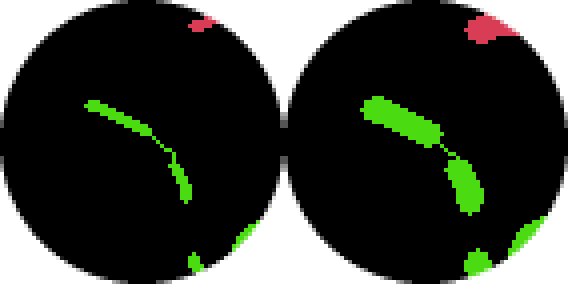
\includegraphics[height=120px]{dilate_example_zoomed_comparison}
	\end{center}
\end{frame}

\begin{frame}[fragile,t]{The experiment}
	\begin{itemize}
		\item With everything dilated with radii 0 through 4, we performed segmentation with the Boykov graph cut segmentation algorithm.
		\item This was performed on all images. There was 2075 label images, with 5 different radii of dilation each for a total of 10375 images to segment.
		\item Analysis is then run on all the segmented images to determine the effects of the dilation.
	\end{itemize}
\end{frame}

\begin{frame}[fragile,t]{The experiment}
	\begin{center}
		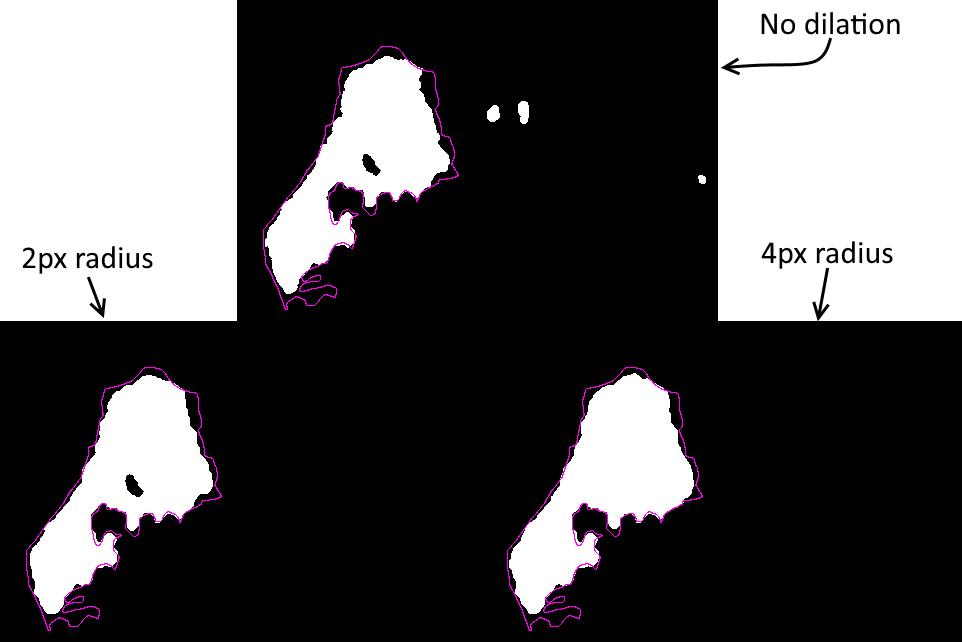
\includegraphics[width=\paperheight]{segmentation_example_all}
	\end{center}
\end{frame}

\begin{frame}[fragile,t]{Segmentation programs}
	\begin{itemize}
		\item We also tried the experiment on a different segmentation program to contrast the differences. The OneCut algorithm was chosen for this.
		\item Adapted an implementation from Lena Gorelick to fit into our pipeline.
		\item The OneCut algorithm seems to be much more sensitive to the amount of user input than the Boykov graph cut algorithm.
		\item Works best where users provided a lot of annotations.
	\end{itemize}
\end{frame}

\begin{frame}[fragile,t]{Segmentation programs}
	\begin{center}
		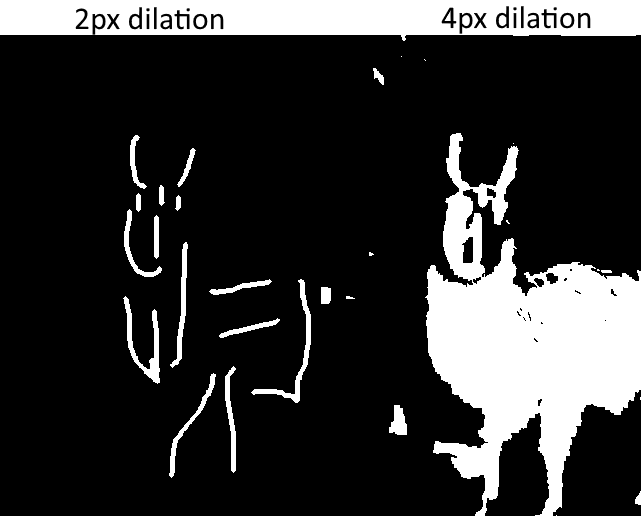
\includegraphics[width=250px]{onecut_segment_comparison}
	\end{center}
\end{frame}

\begin{frame}[fragile,t]{Analyzing accuracy}
	\begin{itemize}
		\item Accuracy in image segmentation is most commonly measured with the Dice Similarity Coefficient.
		\item $\text{DSC} = \frac{2|X \cap Y|}{|X| + |Y|}$
		\item We use this to compare the segmented result to the ground truth.
		\item The value is between 0 and 1, where 0 = no match at all and 1 = perfect match.
	\end{itemize}
\end{frame}

\begin{frame}[fragile,t]{Accuracy results}
	\begin{center}
		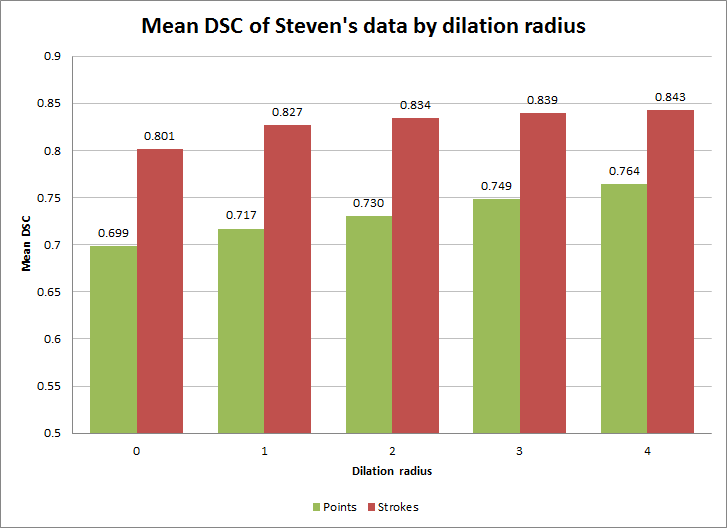
\includegraphics[width=\paperheight]{steven_mean_dsc}
	\end{center}
\end{frame}

\begin{frame}[fragile,t]{Accuracy results}
	\begin{center}
		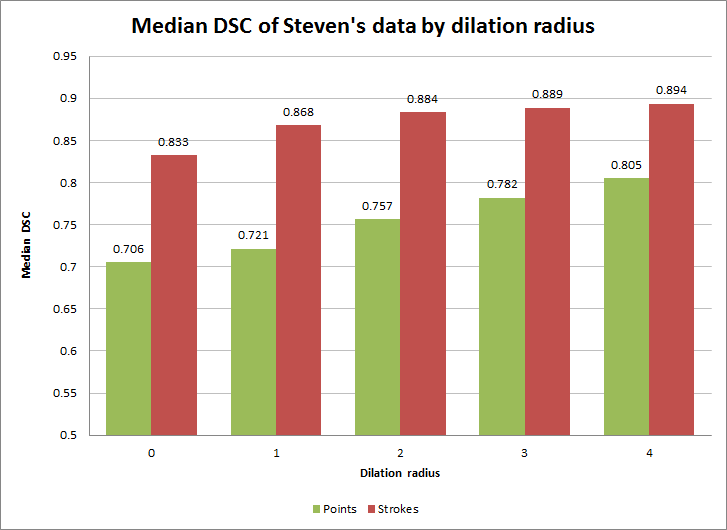
\includegraphics[width=\paperheight]{steven_median_dsc}
	\end{center}
\end{frame}

\begin{frame}[fragile,t]{Accuracy results}
	\begin{center}
		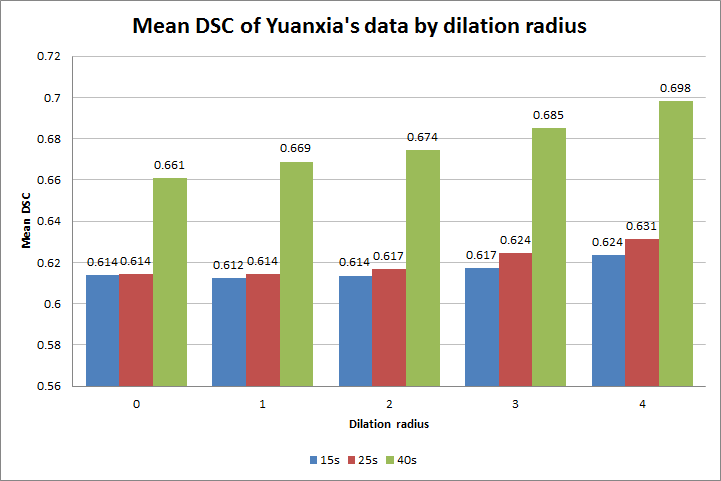
\includegraphics[width=\paperheight]{yuanxia_mean_dsc}
	\end{center}
\end{frame}

\begin{frame}[fragile,t]{Accuracy results}
	\begin{center}
		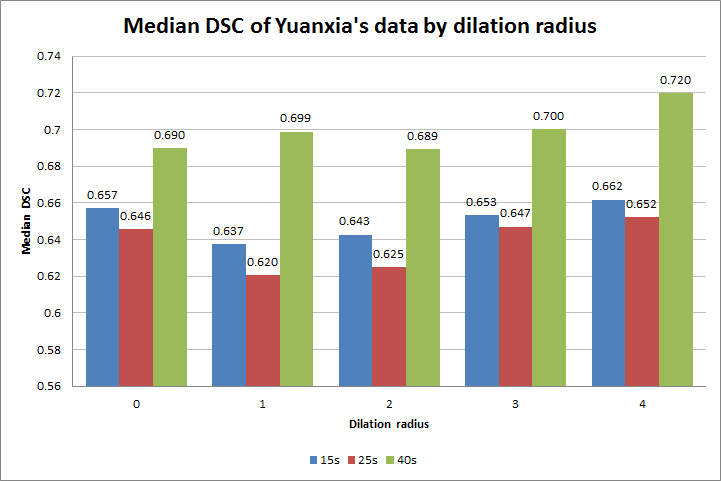
\includegraphics[width=\paperheight]{yuanxia_median_dsc}
	\end{center}
\end{frame}

\begin{frame}[fragile,t]{Accuracy results}
	\begin{center}
		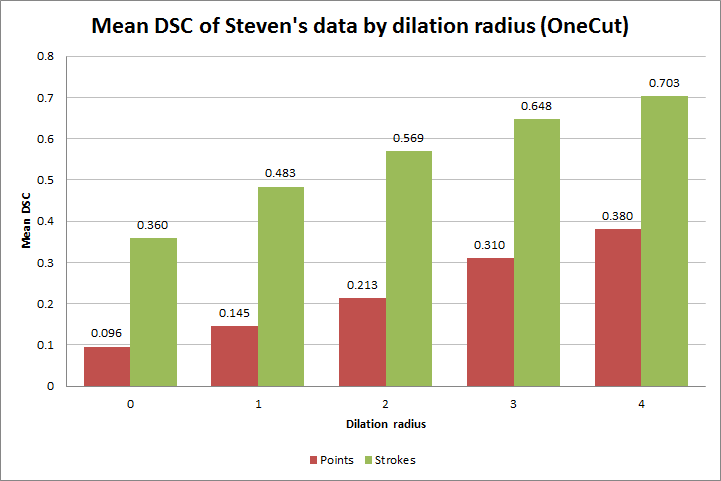
\includegraphics[width=\paperheight]{steven_onecut_dsc}
	\end{center}
\end{frame}

\begin{frame}[fragile,t]{Accuracy results}
	\begin{center}
		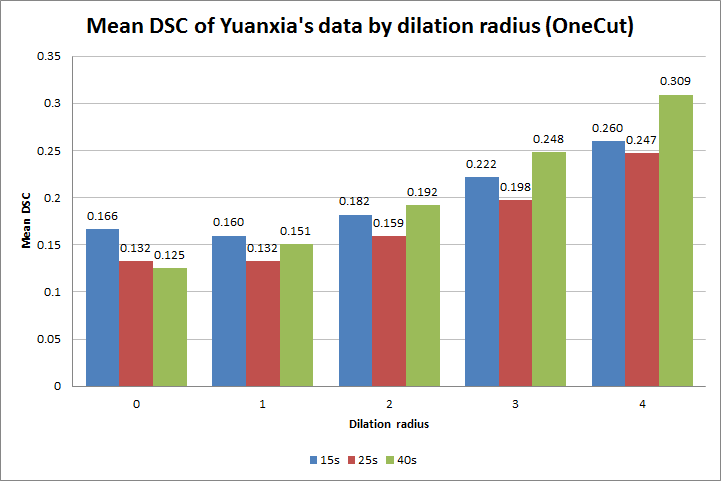
\includegraphics[width=\paperheight]{yuanxia_onecut_dsc}
	\end{center}
\end{frame}

\begin{frame}[fragile,t]{Analyzing reproducibility}
	\begin{itemize}
		\item Reproducibility is a measure of consistency in the segmentation.
		\item We want to know how consistently the algorithm handles different users segmenting the same image.
		\item Measured with the Generalized Tanimoto Coefficient.
		\item $\text{GTC} = \frac{\Sigma \left( X_i \wedge Y_i \right)}{\Sigma \left( X_i \vee Y_i \right)}$
		\item The value is between 0 and 1, where 0 = no consistency between samples and 1 = all samples the same.
	\end{itemize}
\end{frame}

\begin{frame}[fragile,t]{Reproducibility results}
	\begin{center}
		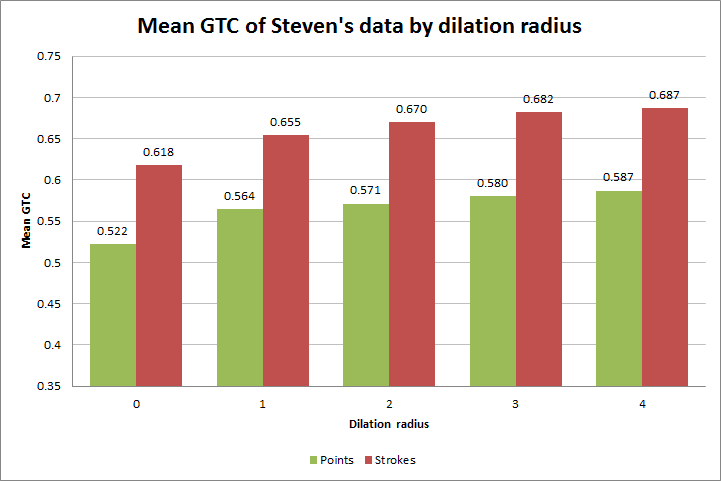
\includegraphics[width=\paperheight]{steven_mean_gtc}
	\end{center}
\end{frame}

\begin{frame}[fragile,t]{Reproducibility results}
	\begin{center}
		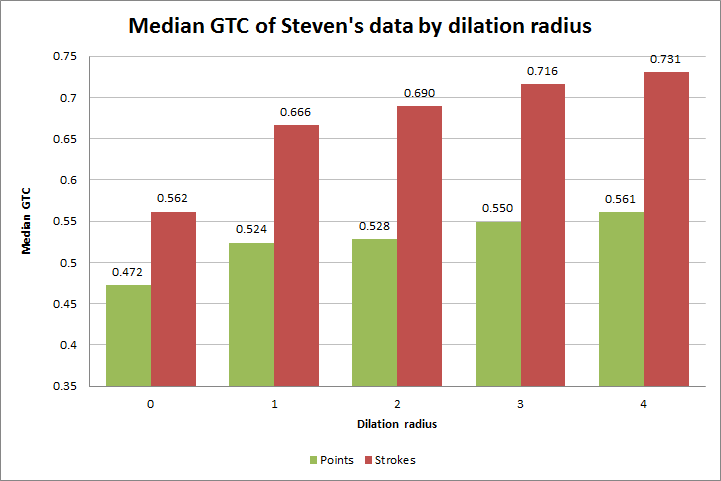
\includegraphics[width=\paperheight]{steven_median_gtc}
	\end{center}
\end{frame}

\begin{frame}[fragile,t]{Reproducibility results}
	\begin{center}
		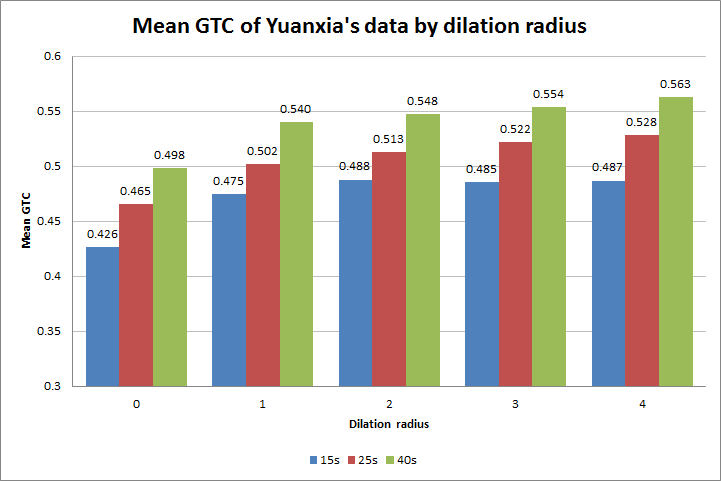
\includegraphics[width=\paperheight]{yuanxia_mean_gtc}
	\end{center}
\end{frame}

\begin{frame}[fragile,t]{Reproducibility results}
	\begin{center}
		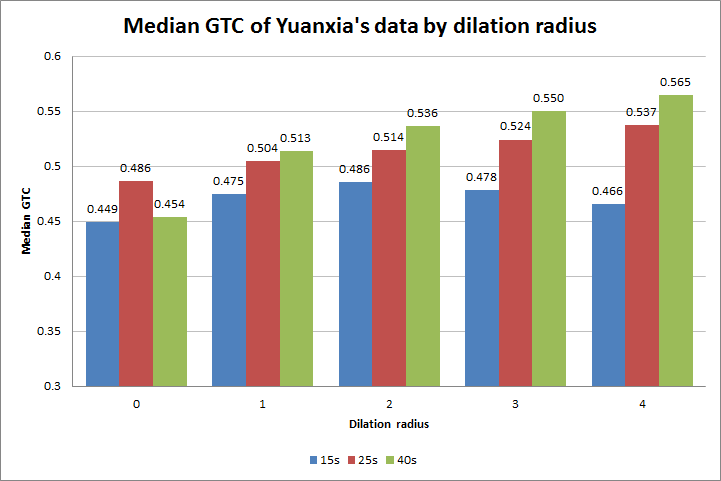
\includegraphics[width=\paperheight]{yuanxia_median_gtc}
	\end{center}
\end{frame}

\begin{frame}[fragile,t]{Reproducibility results}
	\begin{center}
		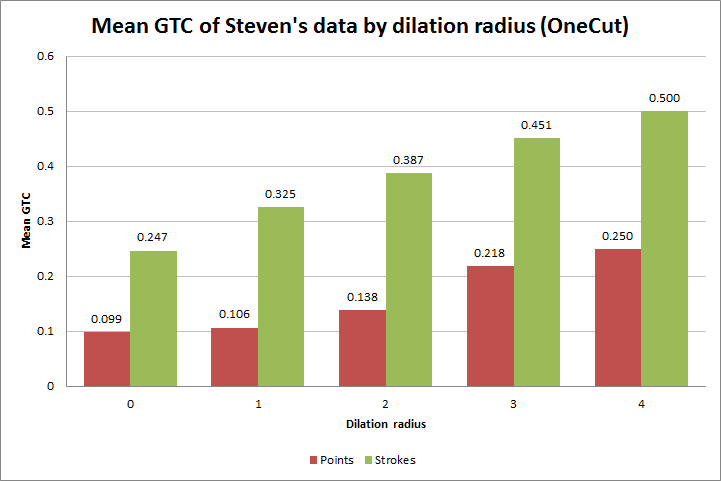
\includegraphics[width=\paperheight]{steven_onecut_gtc}
	\end{center}
\end{frame}

\begin{frame}[fragile,t]{Reproducibility results}
	\begin{center}
		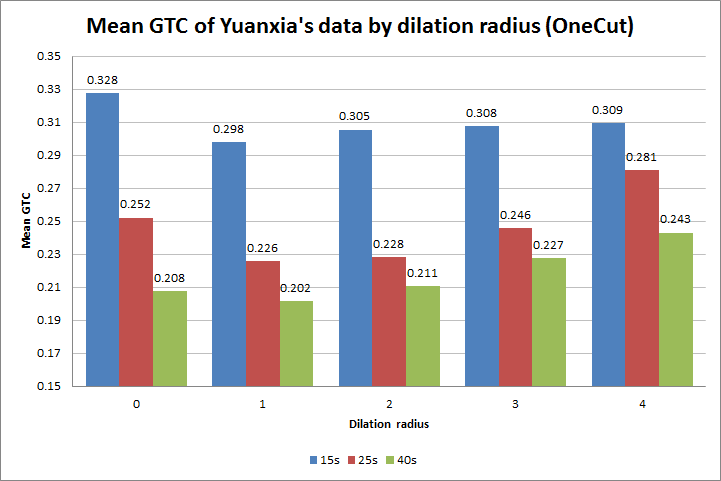
\includegraphics[width=\paperheight]{yuanxia_onecut_gtc}
	\end{center}
\end{frame}

\begin{frame}[fragile,t]{Testing for statistical significance}
	\begin{itemize}
		\item In order to know that our results were statistically significant, we used the Friedman square chi test.
		\item This could only be used within groups of independent variables (eg, no comparing one study's data to another's).
		\item Was chosen because our data was not normally distributed (determined with D'Agostino's $K^2$ test).
		\item Differences statistically significant ($p < 0.01$) for all except Yuanxia's 40s time pressure group for the GTC under OneCut.
	\end{itemize}
\end{frame}

\begin{frame}[fragile,t]{Conclusion}
	\begin{itemize}
		\item Hence, we conclude \textbf{stroke width has a significant impact on our semi-automatic image segmentation programs}.
		\item This can't be generalized for all algorithms. But it seems likely that it may hold for many, or at least not negatively affect accuracy and reproducibility.
		\item The OneCut algorithm's results should be taken with a grain of salt as it often failed to segment in any useful way. However, there was certainly \textit{some} cases where dilation allowed it to achieve a useful segmentation.
	\end{itemize}
\end{frame}

\begin{frame}[fragile,t]{The end}
	Project code and data available at:\\ \footnotesize{\url{https://github.com/KatrinaHoffert/stroke-radius-segmentation}}
	
	\vspace{4em}
	
	\begin{center}
		\huge{Questions?}
	\end{center}
\end{frame}

\end{document}